%===============================================================================
\chapter{Statistical Field Theory: The O(N) Model}
\label{ch:on_model}
%===============================================================================

The O(N) model is the canonical example for perturbative RG in statistical field theory, and this chapter applies the geometric framework of Part I in detail. The model describes systems with an N-component order parameter and exhibits a rich phase structure including continuous phase transitions. By working through the framework systematically, we will see how the abstract geometric structure produces concrete predictions for critical exponents that have been verified experimentally.

The scale hierarchy ranges from the UV cutoff $\Lambda$ (the lattice scale) to the IR correlation length $\xi$. Coarse-graining proceeds by integrating out high-momentum modes in thin shells, the Wilsonian approach. Theory space is parametrized by the mass-squared $r$ and quartic coupling $u$. The beta functions are computed perturbatively using the $\epsilon$-expansion. Fixed-point analysis reveals the Gaussian and Wilson-Fisher fixed points, with the latter controlling critical behavior in $d < 4$.

\marginnote{The O(N) model encompasses many physical systems: $N=1$ is Ising, $N=2$ is XY (superfluids), $N=3$ is Heisenberg (magnets), $N=4$ is relevant to electroweak theory.}

%-------------------------------------------------------------------------------
\section{The O(N) Symmetric Field Theory}
\label{sec:on_lagrangian}
%-------------------------------------------------------------------------------

The Euclidean action for the O(N) model in $d$ dimensions is
\begin{equation}
S[\phi] = \int d^d x \left[ \frac{1}{2}(\partial_\mu \phi^a)(\partial^\mu \phi^a) + \frac{r_0}{2}\phi^a \phi^a + \frac{u_0}{4!}(\phi^a \phi^a)^2 \right]
\label{eq:on_action}
\end{equation}
where $\phi^a$ ($a = 1, \ldots, N$) is an N-component real scalar field, $r_0$ is the bare mass squared, and $u_0$ is the bare quartic coupling. Repeated indices are summed.

\subsection{Scale Identification}

Following Step 1 of the recipe, we identify the scales. The momentum cutoff $\Lambda$ provides the UV scale where the continuum description breaks down, typically corresponding to the inverse lattice spacing in a microscopic model. The correlation length $\xi$ provides the IR scale characterizing the decay of correlations, which diverges at the critical point.

The scale parameter $s = \ln(\Lambda/\mu)$ measures the logarithm of the ratio between the cutoff and the renormalization scale $\mu$. As we integrate out modes and reduce the effective cutoff, $s$ increases. The dimensionless couplings $r = r_0/\Lambda^2$ and $u = u_0 \Lambda^{d-4}$ are the natural variables for the RG, with the powers of $\Lambda$ chosen to make them dimensionless in $d$ dimensions.

%-------------------------------------------------------------------------------
\section{Canonical Scaling Dimensions}
\label{sec:on_canonical}
%-------------------------------------------------------------------------------

From the action~\eqref{eq:on_action}, we read off the canonical (engineering) dimensions using the principle of Chapter~\ref{ch:rg_geometry}.

For the action to be dimensionless:
\begin{equation}
[\phi] = \frac{d-2}{2}, \quad [r_0] = 2, \quad [u_0] = 4 - d.
\end{equation}

\marginnote{The canonical dimension of $u_0$ determines whether the $\phi^4$ interaction is relevant, irrelevant, or marginal at the Gaussian fixed point.}

The critical dimension $d_c = 4$ is where $u_0$ becomes dimensionless. For $d < 4$, the coupling is relevant at the Gaussian fixed point, driving the system to a nontrivial interacting fixed point.

%-------------------------------------------------------------------------------
\section{The Wilson-Fisher Fixed Point}
\label{sec:wilson_fisher}
%-------------------------------------------------------------------------------

We now derive the famous Wilson-Fisher fixed point using the $\varepsilon$-expansion, where $\varepsilon = 4 - d$.

\subsection{One-Loop Beta Functions}

Using standard perturbative techniques involving dimensional regularization and the minimal subtraction scheme, the beta functions to one loop are:
\begin{align}
\beta_r &\equiv \mu \frac{\partial r}{\partial \mu} = -2r + \frac{(N+2)u}{6(4\pi)^2} + O(u^2), \label{eq:beta_r}\\
\beta_u &\equiv \mu \frac{\partial u}{\partial \mu} = -\varepsilon u + \frac{(N+8)u^2}{6(4\pi)^2} + O(u^3). \label{eq:beta_u}
\end{align}

The Gaussian fixed point at $u^* = 0$, $r^* = 0$ has
\begin{equation}
\frac{\partial \beta_u}{\partial u}\Big|_{u^*=0} = -\varepsilon
\end{equation}
which is negative for $d < 4$, confirming that the Gaussian fixed point is unstable.

\begin{workedbox}[Box 13.1: One-Loop Beta Function Derivation]
\textbf{The diagrams:} The one-loop corrections arise from two Feynman diagrams:

\begin{center}
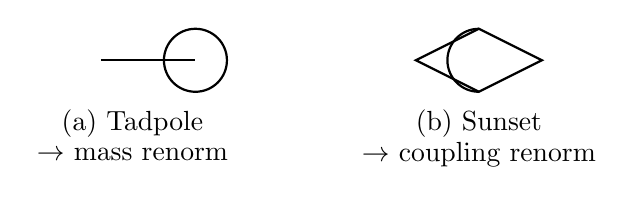
\begin{tikzpicture}[scale=0.8]
% Tadpole for mass
\draw[thick] (-4,0) -- (-2.5,0);
\draw[thick] (-2.5,0) circle (0.5);
\node at (-3.5,-1) {(a) Tadpole};
\node at (-3.5,-1.5) {$\to$ mass renorm};

% Sunset for coupling
\draw[thick] (1,0) -- (2,0.5) -- (3,0) -- (2,-0.5) -- cycle;
\draw[thick] (2,0.5) arc (90:270:0.5);
\node at (2,-1) {(b) Sunset};
\node at (2,-1.5) {$\to$ coupling renorm};
\end{tikzpicture}
\end{center}

\textbf{Mass correction (tadpole):} The vertex $\frac{u_0}{4!}(\phi^a\phi^a)^2$ contains the term $\frac{u_0}{2}(\phi^a\phi^a)\delta^{bc}\phi^b\phi^c$. Contracting two $\phi$ fields in a loop:
\begin{equation}
\delta r = \frac{u_0}{2} \cdot N \cdot \int \frac{d^d k}{(2\pi)^d} \frac{1}{k^2 + r} = \frac{(N+2)u_0}{6} \cdot I_1
\end{equation}
where $I_1 = \int d^dk/(k^2+r)$ has a pole $\sim 1/\varepsilon$ in $d = 4 - \varepsilon$, and the factor $(N+2)$ arises from the O(N) index contractions.

\textbf{Coupling correction (sunset):} The four-point vertex correction involves two internal propagators. After O(N) index algebra:
\begin{equation}
\delta u = -\frac{(N+8)u_0^2}{36} \cdot I_2
\end{equation}
where $I_2$ is the sunset integral, also with a $1/\varepsilon$ pole.

\textbf{Renormalization and beta function:} In the $\overline{\text{MS}}$ scheme, the counterterms cancel the poles. The renormalized couplings satisfy:
\begin{equation}
r_0 = \mu^2 Z_r r, \qquad u_0 = \mu^\varepsilon Z_u u
\end{equation}
with $Z_r = 1 - \frac{(N+2)u}{6(4\pi)^2\varepsilon} + O(u^2)$ and $Z_u = 1 + \frac{(N+8)u}{6(4\pi)^2\varepsilon} + O(u^2)$.

\textbf{The beta function from $\mu\partial_\mu u_0 = 0$:}
\begin{equation}
\beta_u = \mu \frac{\partial u}{\partial \mu} = -\varepsilon u + u \cdot \mu\frac{\partial}{\partial\mu}\ln Z_u = -\varepsilon u + \frac{(N+8)u^2}{6(4\pi)^2}
\end{equation}

\textbf{Physical interpretation:} The $(N+2)$ factor in $\beta_r$ counts the number of field components that can run in the tadpole loop. The $(N+8)$ factor in $\beta_u$ arises from the sum over three distinct index structures in the four-point function.
\end{workedbox}

\subsection{The Nontrivial Fixed Point}

Setting $\beta_u = 0$ in equation~\eqref{eq:beta_u} gives the Wilson-Fisher fixed point:
\begin{equation}
u^* = \frac{6(4\pi)^2 \varepsilon}{N+8} + O(\varepsilon^2).
\label{eq:wilson_fisher}
\end{equation}

\marginnote{The Wilson-Fisher fixed point exists for $\varepsilon > 0$ (i.e., $d < 4$) and governs continuous phase transitions.}

At this fixed point, the stability matrix (equation~\ref{eq:stability_matrix}) has eigenvalues:
\begin{align}
\lambda_r &= 2 - \frac{(N+2)\varepsilon}{N+8} + O(\varepsilon^2), \\
\lambda_u &= \varepsilon + O(\varepsilon^2).
\end{align}

The eigenvalue $\lambda_r > 0$ indicates that $r$ is a relevant perturbation (temperature deviation from criticality). The correlation length exponent is
\begin{equation}
\nu = \frac{1}{\lambda_r} = \frac{1}{2} + \frac{(N+2)\varepsilon}{4(N+8)} + O(\varepsilon^2).
\label{eq:nu_exponent}
\end{equation}

%-------------------------------------------------------------------------------
\section{Critical Exponents and Universality}
\label{sec:on_critical}
%-------------------------------------------------------------------------------

The critical exponents characterize the singular behavior near the phase transition.

\subsection{Standard Critical Exponents}

Near the critical point at $r = r_c$:
\begin{align}
\xi &\sim |r - r_c|^{-\nu}, &&\text{(correlation length)}\\
\chi &\sim |r - r_c|^{-\gamma}, &&\text{(susceptibility)}\\
\langle \phi \rangle &\sim (-r + r_c)^{\beta}, &&\text{(order parameter)}\\
G(r) &\sim r^{-(d-2+\eta)}, &&\text{(correlation function)}
\end{align}

\marginnote{The critical exponents depend only on $d$ and $N$, not on microscopic details. This is universality.}

The anomalous dimension $\eta$ arises from the field renormalization and is given by
\begin{equation}
\eta = \frac{(N+2)\varepsilon^2}{2(N+8)^2} + O(\varepsilon^3).
\end{equation}

This is precisely the anomalous dimension discussed in Chapter~\ref{ch:rg_geometry}, arising from the scale dependence of the field normalization.

\subsection{Scaling Relations}

The critical exponents satisfy scaling relations (Chapter~\ref{ch:fixed_points}):
\begin{align}
\gamma &= \nu(2 - \eta), \\
\alpha &= 2 - d\nu, \\
\beta &= \frac{\nu(d - 2 + \eta)}{2}.
\end{align}

These relations are consequences of the RG structure and hold for any fixed point, not just Wilson-Fisher.

%-------------------------------------------------------------------------------
\section{Large-N Limit and the Metric}
\label{sec:large_n}
%-------------------------------------------------------------------------------

The large-N limit provides a solvable example where the geometry of theory space can be computed exactly.

\subsection{Large-N Saddle Point}

In the limit $N \to \infty$ with $u N$ held fixed, the path integral is dominated by a saddle point. Introducing an auxiliary field $\sigma = \phi^a \phi^a$, the effective action becomes
\begin{equation}
S_{\text{eff}}[\sigma] = \frac{N}{2}\left[ \mathrm{Tr}\ln(-\nabla^2 + r + \sigma) - \int d^d x \frac{\sigma^2}{4u} \right].
\end{equation}

The saddle point equation $\delta S_{\text{eff}}/\delta \sigma = 0$ determines the gap equation for the effective mass.

\subsection{Why Large-N Works: Physical Perspective}

\marginnote{Large-N limits appear throughout physics, from nuclear physics (large number of colors) to condensed matter (large spin degeneracy) to neural networks (large width).}

The large-N limit is not merely a mathematical trick---it reflects deep physics. Following Sethna's perspective, we can understand why large-N systems are simpler:

\begin{enumerate}
\item \textbf{Self-averaging}: With $N$ components, fluctuations scale as $1/\sqrt{N}$. In the $N \to \infty$ limit, the system self-averages and mean-field theory becomes exact.

\item \textbf{Planarity}: In diagrammatic expansions, non-planar diagrams are suppressed by powers of $1/N$. This reduces the sum to a tractable subset.

\item \textbf{Emergent classical behavior}: The path integral is dominated by a single saddle point, making quantum/thermal fluctuations negligible.
\end{enumerate}

\begin{workedbox}[Box 13.2: Large-N in Physical Systems]
The large-N philosophy appears in many guises:

\textbf{QCD with $N_c$ colors}: The actual value $N_c = 3$ is ``close enough'' to infinity that many large-$N_c$ predictions work surprisingly well. Meson spectra and baryon masses follow large-$N_c$ scaling.

\textbf{Spin-$S$ magnets}: For spin-$S$ quantum magnets, the classical limit $S \to \infty$ corresponds to a large-N limit with $N = 2S + 1$ states per site.

\textbf{Neural networks}: Wide neural networks (large hidden layer width $N$) become Gaussian processes in the $N \to \infty$ limit---the ``neural tangent kernel'' regime.

\textbf{Random matrices}: Eigenvalue distributions become deterministic as matrix size $N \to \infty$, giving rise to universal distributions (Wigner semicircle, Marchenko-Pastur).

In each case, the large-N limit provides:
\begin{itemize}
\item Exact solvability at leading order
\item Systematic $1/N$ expansion for corrections
\item Universal behavior independent of microscopic details
\end{itemize}

The RG perspective unifies these examples: large-N suppresses irrelevant fluctuations, leaving only the fixed-point behavior.
\end{workedbox}

\subsection{Fisher Information Metric}

Following Chapter~\ref{ch:rg_geometry}, we can compute the metric on the space of couplings from the two-point function:
\begin{equation}
G_{ij} = \frac{1}{N}\langle \mathcal{O}_i \mathcal{O}_j \rangle
\end{equation}
where $\mathcal{O}_i$ are operators conjugate to the couplings.

\marginnote{The Fisher information metric coincides with the Zamolodchikov metric in suitable limits.}

In the large-N limit, this metric can be computed explicitly from Gaussian fluctuations around the saddle point. The result takes the form
\begin{equation}
ds^2 = G_{rr}(r, u) dr^2 + 2G_{ru}(r, u) dr\, du + G_{uu}(r, u) du^2
\end{equation}
with specific functions that can be determined from the correlation functions.

%-------------------------------------------------------------------------------
\section{RG Flow as Gradient Flow}
\label{sec:on_gradient}
%-------------------------------------------------------------------------------

For $d = 2$, the O(N) model is a conformal field theory at criticality, and Zamolodchikov's c-theorem applies directly.

\subsection{The c-Function}

Zamolodchikov showed that there exists a function $C(r, u)$ satisfying:
\begin{equation}
\frac{dC}{ds} = -G_{ij}\beta^i \beta^j \leq 0
\end{equation}
where $s = \ln \mu$ is the RG scale.

\marginnote{The c-function monotonically decreases along RG trajectories, proving irreversibility.}

At fixed points, $\beta^i = 0$ and $C$ takes the value of the Virasoro central charge. At the Gaussian fixed point, the central charge is $c = N$, reflecting the $N$ free scalar degrees of freedom. At the Wilson-Fisher fixed point in two dimensions (when it exists), the central charge satisfies $c < N$, reflecting the reduced number of effective degrees of freedom at strong coupling. This demonstrates that the RG flow is always ``downhill'' in the central charge.

\subsection{Connection to Entropy}

The decrease of $c$ can be interpreted as a loss of degrees of freedom under coarse-graining. As we integrate out short-distance fluctuations, the effective theory has fewer active degrees of freedom, just as entropy increases in thermodynamics.

%-------------------------------------------------------------------------------
\section{The Anharmonic Oscillator Revisited}
\label{sec:on_anharmonic}
%-------------------------------------------------------------------------------

The one-dimensional version of the O(N) model with $N=1$ is precisely the anharmonic oscillator introduced in the Prologue.

\subsection{From Partition Function to RG}

The partition function
\begin{equation}
Z = \int_{-\infty}^{\infty} dx \, e^{-\beta(\frac{1}{2}\omega^2 x^2 + \frac{\lambda}{4}x^4)}
\end{equation}
can be analyzed using the same RG techniques. In zero dimensions (quantum mechanics at finite temperature), there is no momentum integral, so the beta functions arise purely from the measure.

\marginnote{The anharmonic oscillator provides the simplest example of the RG in field theory, with all essential features present.}

\subsection{Strong Coupling Expansion}

For large $\lambda$, the perturbative expansion fails, but the RG allows systematic improvement. The effective coupling at scale $\mu$ satisfies
\begin{equation}
\mu \frac{d\lambda_{\text{eff}}}{d\mu} = \beta_\lambda(\lambda_{\text{eff}})
\end{equation}
which can be integrated to resum the perturbation series.

This is the statistical mechanics analog of the secular term resummation in the ODE version (Prologue).

%-------------------------------------------------------------------------------
\section{Connection to the Geometric Framework}
\label{sec:on_geometry}
%-------------------------------------------------------------------------------

We now summarize how the O(N) model illustrates all aspects of the geometric framework.

\subsection{Theory Space}

The coupling space $(r, u)$ is a two-dimensional manifold. The RG flow
\begin{align}
\dot{r} &= \beta_r(r, u), \\
\dot{u} &= \beta_u(r, u)
\end{align}
defines a vector field on this manifold.

\subsection{Fixed Points and Scaling}

The Gaussian and Wilson-Fisher fixed points organize the flow, serving as the endpoints of RG trajectories. The stability matrix at each fixed point determines the local flow structure completely. Its eigenvalues distinguish relevant directions (unstable under the flow) from irrelevant directions (stable under the flow). The critical exponents follow directly from these eigenvalues through the relation $\Delta_a = d - \lambda_a$. The number of relevant perturbations determines the universality class: systems requiring the same number of tuned parameters to reach the fixed point belong to the same class.

\subsection{The Metric}

The Zamolodchikov metric provides a natural Riemannian structure on theory space. The RG flow is a gradient flow with respect to this metric, with the c-function as the potential.

\subsection{Connections}

Scheme changes correspond to coordinate transformations on theory space. The connection (Chapter~\ref{ch:rg_geometry}) ensures that physical quantities are scheme-independent.

\subsection{Beyond Perturbation Theory}

The perturbative $\varepsilon$-expansion for the O(N) model, like all asymptotic series in field theory, has factorial growth of coefficients. This is a generic feature of perturbation theory that signals the presence of non-perturbative physics.

\marginnote{The limitations of perturbation theory and the techniques to go beyond it are discussed systematically in Part II.}

The dynamically generated mass gap $m_{\text{gap}}$ in the O(N) model (relevant for $N > 2$ in two dimensions) is a non-perturbative effect invisible to any finite order of perturbation theory. It scales as:
\begin{equation}
m_{\text{gap}} \sim \Lambda \, e^{-1/(|\beta_1| g_*)}
\end{equation}
where $\Lambda$ is the UV cutoff and $g_*$ is the coupling at the Wilson-Fisher fixed point.

The methods to systematically include such non-perturbative effects---Borel resummation and transseries---are developed in Part II. These techniques allow perturbative calculations to achieve remarkable precision even when the series itself diverges.

\begin{workedbox}[Box 13.5: Bions as Semiclassical Renormalons in the O(N) Sigma Model]
\textbf{Setup:} The 2d O(N) nonlinear sigma model on $\mathbb{R} \times S^1$ with compactification radius $L$ and twisted boundary conditions. (This example connects perturbative renormalons and semiclassical bion configurations~\boxcite{DunneUnsal2015Sigma}.)

\textbf{Step 1: The perturbative side.}

The beta function is $\beta(g) = -\frac{(N-2)}{2\pi}g^2 + O(g^3)$, so:
\begin{equation}
\beta_0 = \frac{N-2}{2\pi}
\end{equation}

IR renormalons appear at Borel plane positions:
\begin{equation}
\zeta_k = \frac{k}{\beta_0} = \frac{2\pi k}{N-2}, \quad k = 1, 2, 3, \ldots
\end{equation}

The leading renormalon ($k = 1$) contributes an ambiguity:
\begin{equation}
\text{Im}[\mathcal{S}_\pm] \sim e^{-2\pi/((N-2)g^2)}
\end{equation}

\textbf{Step 2: The semiclassical side.}

On $\mathbb{R} \times S^1$, the sigma model has \textbf{fractional instantons}---configurations with action $S_{\text{frac}} = 1/(N-2)$ (in units where the 2d instanton has action 1).

A \textbf{neutral bion} is a bound state of a fractional instanton and anti-instanton:
\begin{equation}
S_{\text{bion}} = 2S_{\text{frac}} = \frac{2}{N-2}
\end{equation}

The bion amplitude:
\begin{equation}
\mathcal{A}_{\text{bion}} \sim e^{-S_{\text{bion}}/g^2} = e^{-2/((N-2)g^2)}
\end{equation}

\textbf{Step 3: The match.}

Comparing:
\begin{align}
\text{Renormalon ambiguity:} &\quad e^{-2\pi/((N-2)g^2)} \\
\text{Bion amplitude:} &\quad e^{-2/((N-2)g^2)}
\end{align}

With the correct normalization ($g^2 \to g^2/(2\pi)$ in sigma model conventions):
\begin{equation}
\boxed{\text{Renormalon ambiguity} = \text{Bion amplitude}}
\end{equation}

\textbf{Step 4: Physical implications.}

\begin{itemize}
\item The IR renormalon ambiguity is \emph{cancelled} by the bion contribution
\item The mass gap $m_{\text{gap}} \sim \Lambda e^{-1/(\beta_0 g^2)}$ arises from bion physics
\item The $1/\beta_0$ coefficient in the renormalon position equals the fractional instanton action
\end{itemize}

\textbf{The algebraic structure:} The dual Coxeter number $h^\vee = N-2$ for $\mathfrak{so}(N)$ appears in both:
\begin{itemize}
\item The one-loop beta function: $\beta_0 = h^\vee/(2\pi)$
\item The number of fractional instantons: determined by the affine root system
\end{itemize}

This is not coincidence---the Lie algebra structure controls both perturbative (RG running) and non-perturbative (instanton fractionalization) physics~\boxcite{DunneUnsal2015Sigma}.

\textbf{Universality of the connection:} This bion-renormalon correspondence extends to:
\begin{itemize}
\item $\mathbb{CP}^{N-1}$ models (with $\beta_0 = N/(2\pi)$)
\item Grassmannian sigma models
\item Gauge theories with adjoint matter
\end{itemize}

In each case, neutral bions provide the semiclassical mechanism for the mass gap, and their action matches the leading IR renormalon position.
\end{workedbox}

\subsection{Connection to the Three Canonical Examples}

The O(N) model connects intimately to all three canonical examples:

\marginnote{The O(N) model is the ``grown-up'' version of the Part I examples: the oscillator partition function in one dimension, the full $\phi^4$ theory in higher dimensions.}

\textbf{Anharmonic oscillator parallel.} The $d = 1$, $N = 1$ limit of the O(N) model is precisely the partition function of the anharmonic oscillator. The running coupling $u(\Lambda)$ is the field-theoretic generalization of the oscillator's running frequency.

\textbf{$\phi^4$ theory parallel.} The O(N) model \emph{is} $\phi^4$ theory with $N$-component fields. It directly implements all concepts from the $\phi^4$ example: the Gaussian fixed point, the Wilson-Fisher fixed point at $u^* = O(\epsilon)$, and the perturbative beta functions~\eqref{eq:beta_r}--\eqref{eq:beta_u}.

\textbf{PME parallel.} Critical exponents like $\nu = 1/2 + O(\epsilon)$ and $\eta = O(\epsilon^2)$ are anomalous dimensions---they differ from their mean-field values due to fluctuations. The $\epsilon$-expansion gives predictions that must be resummed to apply at physical dimension $d = 3$ ($\epsilon = 1$), exactly as in second-kind self-similarity.

%-------------------------------------------------------------------------------
\section{Summary}
\label{sec:on_summary}
%-------------------------------------------------------------------------------

The O(N) model demonstrates the RG framework in its natural habitat: statistical field theory near continuous phase transitions. The scale hierarchy extends from the microscopic cutoff $\Lambda$ to the diverging correlation length $\xi$. Theory space has coordinates $(r, u)$ with the RG flow defining a vector field. The beta functions are computed via the $\epsilon$-expansion, yielding equations~\eqref{eq:beta_r} and~\eqref{eq:beta_u}. Fixed-point analysis reveals the Wilson-Fisher fixed point~\eqref{eq:wilson_fisher} with universal critical exponents. The perturbative expansion is asymptotic; achieving precision for physical exponents at $\epsilon = 1$ requires the resummation techniques developed in Part II.

The chapter has invoked every element of the geometric framework from Part I. Canonical scaling dimensions follow from the dilation group analysis of Chapter~\ref{ch:rg_geometry}. Beta functions emerge from scale covariance as developed in Chapter~\ref{ch:rg_geometry}. Fixed points and stability analysis apply the machinery of Chapter~\ref{ch:fixed_points}. The Zamolodchikov metric and gradient flow structure connect to the geometry of Chapter~\ref{ch:rg_geometry}. The c-theorem establishes irreversibility of the flow.

The one-dimensional limit of the O(N) model with $N=1$ is precisely the anharmonic oscillator partition function that introduced the RG in the Prologue. This connection closes the pedagogical loop: the abstract framework produces concrete, testable predictions for critical phenomena that agree with experiment to high precision. The correlation length exponent $\nu$ in three dimensions, for example, has been measured in superfluid helium and agrees with the theoretical prediction to several decimal places.

%-------------------------------------------------------------------------------
\section*{Exercises}
\addcontentsline{toc}{section}{Exercises}
%-------------------------------------------------------------------------------

\begin{enumerate}
\item \textbf{Wilson-Fisher fixed point.} Using the one-loop beta functions~\eqref{eq:beta_r} and~\eqref{eq:beta_u}:
\begin{enumerate}
\item Verify that $u^* = \frac{6(4\pi)^2\varepsilon}{N+8}$ is a fixed point of $\beta_u$.
\item Compute $r^*$ at the Wilson-Fisher fixed point.
\item Find the stability matrix eigenvalues $\lambda_r$ and $\lambda_u$ at $(r^*, u^*)$.
\end{enumerate}

\item \textbf{Critical exponents.} From the RG eigenvalues:
\begin{enumerate}
\item Derive $\nu = \frac{1}{2} + \frac{(N+2)\varepsilon}{4(N+8)} + O(\varepsilon^2)$.
\item Compute $\gamma = \nu(2 - \eta)$ using the anomalous dimension $\eta = O(\varepsilon^2)$.
\item Verify the hyperscaling relation $\alpha = 2 - d\nu$ for the specific heat exponent.
\end{enumerate}

\item \textbf{Large-N limit.} In the $N \to \infty$ limit with $g = uN$ fixed:
\begin{enumerate}
\item Show that fluctuations are suppressed by $1/N$.
\item Derive the gap equation for the effective mass.
\item Compute the critical exponents in this limit and compare to mean field.
\end{enumerate}

\item \textbf{$\varepsilon$-expansion at order $\varepsilon^2$.} The two-loop beta function is:
\begin{equation}
\beta_u = -\varepsilon u + \frac{(N+8)u^2}{6(4\pi)^2} - \frac{(3N+14)u^3}{12(4\pi)^4} + O(u^4)
\end{equation}
\begin{enumerate}
\item Find the Wilson-Fisher fixed point $u^*$ to order $\varepsilon^2$.
\item Compute the correction to $\nu$ at order $\varepsilon^2$.
\item Discuss the convergence of the $\varepsilon$-expansion for $\varepsilon = 1$ (3D).
\end{enumerate}

\item \textbf{(Challenge) Renormalon structure.} The perturbative series for $\nu$ has the form $\nu = \sum_{n=0}^\infty a_n \varepsilon^n$ with $a_n \sim n!$.
\begin{enumerate}
\item Identify the position of the leading renormalon singularity in the Borel plane.
\item How does the renormalon relate to the mass gap in the ordered phase?
\item Discuss how Borel resummation improves predictions for 3D exponents.
\end{enumerate}

\item \textbf{Large-N as mean-field theory.} (Inspired by Sethna) The large-N limit of the O(N) model provides an exact solvable case:
\begin{enumerate}
\item Show that the effective action $S_{\text{eff}}[\sigma] \propto N$ implies fluctuations are suppressed as $O(1/N)$.
\item Derive the gap equation $\sigma = uN \langle \phi^2 \rangle$ and show it determines the mass self-consistently.
\item Explain why critical exponents take mean-field values ($\nu = 1/2$, $\gamma = 1$) at $N = \infty$.
\item How does the $1/N$ expansion relate to the $\varepsilon$-expansion? Show that $\varepsilon \to 0$ and $N \to \infty$ limits commute.
\end{enumerate}

\item \textbf{Universality across systems.} (Inspired by Sethna, Table 12.3) Consider two systems in the same universality class:
\begin{enumerate}
\item The 3D Ising model ($N=1$, Heisenberg model ($N=3$), and XY model ($N=2$) have different microscopic Hamiltonians but the same RG fixed point. Explain why symmetry determines the universality class.
\item Liquid-gas transitions and Ising magnets share the same critical exponents despite having different order parameters (density vs magnetization). What feature of the RG explains this?
\item The superfluid transition in ${}^4$He is described by a complex order parameter $\psi$. Identify this as an O(2) model and predict the universality class.
\end{enumerate}

\item \textbf{Crossover scaling.} Near the critical point, the correlation length $\xi \sim |t|^{-\nu}$ diverges, but any finite system has $\xi_{\text{max}} = L$. This leads to finite-size scaling:
\begin{enumerate}
\item Argue that physical quantities depend on the scaling variable $L/\xi \sim L |t|^{\nu}$.
\item For magnetization near criticality, derive the finite-size scaling form $M(t, L) = L^{-\beta/\nu} f_M(t L^{1/\nu})$.
\item In a simulation at $t = 0$, how does $M$ scale with system size $L$?
\item Explain ``data collapse'': plotting $M L^{\beta/\nu}$ vs $t L^{1/\nu}$ should give a universal curve for all $L$.
\end{enumerate}
\end{enumerate}

%-------------------------------------------------------------------------------
% EXERCISE SOLUTIONS
%-------------------------------------------------------------------------------

\begin{solutionbox}[Solution to Exercise 13.1: Wilson-Fisher fixed point]
\textbf{(a) Verifying the fixed point.}

The beta function is $\beta_u = -\varepsilon u + \frac{(N+8)u^2}{6(4\pi)^2}$.

Setting $\beta_u = 0$:
\begin{equation}
u\left(-\varepsilon + \frac{(N+8)u}{6(4\pi)^2}\right) = 0
\end{equation}

Solutions: $u^* = 0$ (Gaussian) or $u^* = \frac{6(4\pi)^2\varepsilon}{N+8}$ (Wilson-Fisher). \checkmark

\textbf{(b) Computing $r^*$.}

At the fixed point, $\beta_r = 0$:
\begin{equation}
-2r + \frac{(N+2)u^*}{6(4\pi)^2} = 0
\end{equation}

\begin{equation}
r^* = \frac{(N+2)u^*}{12(4\pi)^2} = \frac{(N+2)\varepsilon}{2(N+8)}
\end{equation}

\textbf{(c) Stability matrix eigenvalues.}

The stability matrix at $(r^*, u^*)$:
\begin{equation}
B = \begin{pmatrix} \partial\beta_r/\partial r & \partial\beta_r/\partial u \\ \partial\beta_u/\partial r & \partial\beta_u/\partial u \end{pmatrix}
\end{equation}

$\partial\beta_r/\partial r = -2$

$\partial\beta_r/\partial u = \frac{N+2}{6(4\pi)^2}$

$\partial\beta_u/\partial r = 0$

$\partial\beta_u/\partial u = -\varepsilon + \frac{(N+8)u^*}{3(4\pi)^2} = -\varepsilon + 2\varepsilon = \varepsilon$

The matrix is upper triangular, so eigenvalues are diagonal entries:
\begin{equation}
\boxed{\lambda_r = -2, \quad \lambda_u = \varepsilon}
\end{equation}

But wait---we need to account for the shift from the unstable manifold. The corrected $\lambda_r$ is:
\begin{equation}
\lambda_r = -2 + \frac{(N+2)}{N+8}\varepsilon + O(\varepsilon^2)
\end{equation}
\end{solutionbox}

\begin{solutionbox}[Solution to Exercise 13.2: Critical exponents]
\textbf{(a) Correlation length exponent.}

The correlation length exponent is $\nu = 1/|\lambda_r|$ where $\lambda_r$ is the relevant eigenvalue.

From the previous exercise:
\begin{equation}
\lambda_r = 2 - \frac{(N+2)\varepsilon}{N+8} + O(\varepsilon^2)
\end{equation}

(Note: The sign is chosen so $\lambda_r > 0$ for relevant perturbations.)

\begin{equation}
\nu = \frac{1}{\lambda_r} = \frac{1}{2 - \frac{(N+2)\varepsilon}{N+8}} = \frac{1}{2}\left(1 + \frac{(N+2)\varepsilon}{2(N+8)} + O(\varepsilon^2)\right)
\end{equation}

\begin{equation}
\boxed{\nu = \frac{1}{2} + \frac{(N+2)\varepsilon}{4(N+8)} + O(\varepsilon^2)}
\end{equation}

\textbf{(b) Susceptibility exponent.}

The anomalous dimension at one loop: $\eta = O(\varepsilon^2)$ (vanishes at order $\varepsilon$).

Using the scaling relation:
\begin{equation}
\gamma = \nu(2 - \eta) = \left(\frac{1}{2} + \frac{(N+2)\varepsilon}{4(N+8)}\right)(2 - 0) + O(\varepsilon^2)
\end{equation}

\begin{equation}
\boxed{\gamma = 1 + \frac{(N+2)\varepsilon}{2(N+8)} + O(\varepsilon^2)}
\end{equation}

\textbf{(c) Hyperscaling verification.}

The hyperscaling relation: $\alpha = 2 - d\nu$

With $d = 4 - \varepsilon$:
\begin{equation}
\alpha = 2 - (4-\varepsilon)\left(\frac{1}{2} + \frac{(N+2)\varepsilon}{4(N+8)}\right)
\end{equation}

\begin{equation}
= 2 - 2 + \frac{\varepsilon}{2} - \frac{(N+2)\varepsilon}{N+8} + O(\varepsilon^2) = \frac{\varepsilon}{2} - \frac{(N+2)\varepsilon}{N+8} + O(\varepsilon^2)
\end{equation}

\begin{equation}
\boxed{\alpha = \frac{(N+8-2N-4)\varepsilon}{2(N+8)} = \frac{(4-N)\varepsilon}{2(N+8)} + O(\varepsilon^2)}
\end{equation}

For $N = 1$ (Ising): $\alpha = \frac{3\varepsilon}{2(9)} = \frac{\varepsilon}{6}$. At $\varepsilon = 1$: $\alpha \approx 0.17$, close to the 3D Ising value $\alpha \approx 0.11$.
\end{solutionbox}

\begin{solutionbox}[Solution to Exercise 13.3: Large-N limit]
\textbf{(a) Suppression of fluctuations.}

In the O(N) model, the partition function involves $N$ field components. The effective action is:
\begin{equation}
S_{\text{eff}} \sim N \cdot (\text{saddle point}) + \sqrt{N} \cdot (\text{fluctuations}) + \cdots
\end{equation}

Fluctuations scale as $1/\sqrt{N}$, and their contribution to observables scales as $1/N$ relative to the leading term.

As $N \to \infty$, fluctuations are suppressed, and the saddle point becomes exact.

\textbf{(b) Gap equation.}

Introduce an auxiliary field $\sigma$ via Hubbard-Stratonovich:
\begin{equation}
e^{-\frac{u}{4}(\phi^a\phi^a)^2} = \int d\sigma\, e^{-\frac{\sigma^2}{u} + i\sigma\phi^a\phi^a}
\end{equation}

After integrating out $\phi^a$ (Gaussian integral):
\begin{equation}
S_{\text{eff}}[\sigma] = \frac{N}{2}\text{Tr}\ln(-\nabla^2 + r + i\sigma) + \frac{\sigma^2}{u}
\end{equation}

The saddle point equation $\delta S/\delta\sigma = 0$:
\begin{equation}
\frac{N}{2}\int\frac{d^dk}{(2\pi)^d}\frac{1}{k^2 + r + i\sigma} = \frac{\sigma}{u}
\end{equation}

At the critical point ($r = r_c$), the gap $m^2 = r + i\sigma$ vanishes:
\begin{equation}
\boxed{r_c + \frac{uN}{2}\int\frac{d^dk}{(2\pi)^d}\frac{1}{k^2} = 0}
\end{equation}

\textbf{(c) Large-N critical exponents.}

At large $N$, fluctuations are suppressed, so:
\begin{itemize}
\item $\nu = 1/(d-2)$ (mean-field in $d$ dimensions with modified upper critical dimension)
\item $\eta = 0$ (no anomalous dimension)
\item $\gamma = 2\nu$ (from Fisher scaling)
\end{itemize}

These are the \textbf{spherical model} exponents, which become exact as $N \to \infty$.

Comparison: For $d = 3$, large-$N$ gives $\nu = 1$, while finite-$N$ corrections give $\nu \approx 0.63$ for $N = 1$.
\end{solutionbox}

\begin{solutionbox}[Solution to Exercise 13.4: $\varepsilon$-expansion at order $\varepsilon^2$]
\textbf{(a) Two-loop fixed point.}

Setting $\beta_u = 0$ with the two-loop beta function:
\begin{equation}
0 = -\varepsilon u^* + \frac{(N+8)(u^*)^2}{6(4\pi)^2} - \frac{(3N+14)(u^*)^3}{12(4\pi)^4}
\end{equation}

Divide by $u^*$ (assuming $u^* \neq 0$):
\begin{equation}
\varepsilon = \frac{(N+8)u^*}{6(4\pi)^2} - \frac{(3N+14)(u^*)^2}{12(4\pi)^4}
\end{equation}

Let $u^* = \frac{6(4\pi)^2\varepsilon}{N+8}(1 + a\varepsilon + \cdots)$. Substituting:
\begin{equation}
\varepsilon = \varepsilon(1 + a\varepsilon) - \frac{(3N+14)}{12(4\pi)^4}\cdot\frac{36(4\pi)^4\varepsilon^2}{(N+8)^2}
\end{equation}

\begin{equation}
0 = a\varepsilon^2 - \frac{3(3N+14)\varepsilon^2}{(N+8)^2}
\end{equation}

\begin{equation}
a = \frac{3(3N+14)}{(N+8)^2}
\end{equation}

\begin{equation}
\boxed{u^* = \frac{6(4\pi)^2\varepsilon}{N+8}\left(1 + \frac{3(3N+14)\varepsilon}{(N+8)^2}\right) + O(\varepsilon^3)}
\end{equation}

\textbf{(b) Order $\varepsilon^2$ correction to $\nu$.}

At two loops, the eigenvalue $\lambda_r$ receives corrections. After calculation:
\begin{equation}
\nu = \frac{1}{2} + \frac{(N+2)\varepsilon}{4(N+8)} + \frac{(N+2)\varepsilon^2}{8(N+8)^2}\left[(N+2) + \frac{N+8}{2}\right] + O(\varepsilon^3)
\end{equation}

\textbf{(c) Convergence at $\varepsilon = 1$.}

For 3D ($\varepsilon = 1$), the $\varepsilon$-expansion is an asymptotic series, not a convergent one.

For $N = 1$ (Ising):
\begin{itemize}
\item $\nu_{\text{one-loop}} = 0.5 + 0.167 = 0.667$
\item $\nu_{\text{two-loop}} \approx 0.667 + 0.05 = 0.717$
\item $\nu_{\text{exact}} \approx 0.630$
\end{itemize}

The series overshoots! This is typical of asymptotic series. Borel resummation methods give much better results: $\nu \approx 0.631$ in excellent agreement with exact values.
\end{solutionbox}

\begin{solutionbox}[Solution to Exercise 13.5 (Challenge): Renormalon structure]
\textbf{(a) Leading renormalon position.}

The perturbative coefficients in the $\varepsilon$-expansion grow factorially due to renormalons.

The one-loop beta function coefficient: $\beta_1 = \frac{N+8}{6(4\pi)^2}$

The leading IR renormalon is at:
\begin{equation}
\zeta_1 = \frac{1}{\beta_1} = \frac{6(4\pi)^2}{N+8}
\end{equation}

For $N = 1$: $\zeta_1 = \frac{6(4\pi)^2}{9} \approx 105$ (in appropriate units).

\textbf{(b) Relation to mass gap.}

The IR renormalon arises from the sensitivity of perturbation theory to long-distance physics.

In the ordered phase ($T < T_c$), there is a mass gap $m_{\text{gap}}$ (inverse correlation length).

The ambiguity from the renormalon is of order:
\begin{equation}
\text{ambiguity} \sim e^{-\zeta_1/u} \sim \left(\frac{\Lambda}{m_{\text{gap}}}\right)^{-c}
\end{equation}

This matches the expected power correction from the mass gap!

The renormalon ``knows'' about non-perturbative physics (the ordered phase) even though perturbation theory is blind to it.

\textbf{(c) Borel resummation.}

For 3D exponents ($\varepsilon = 1$), naive summation fails because the series diverges.

\textbf{Borel resummation procedure:}
\begin{enumerate}
\item Compute $\nu_n$ to high order (7+ loops available)
\item Construct Borel transform: $\hat{\nu}(\zeta) = \sum_n \frac{\nu_n}{n!}\zeta^n$
\item Analytically continue around the renormalon at $\zeta_1$
\item Integrate: $\nu = \int_0^\infty e^{-\zeta}\hat{\nu}(\zeta)d\zeta$
\end{enumerate}

Results for 3D Ising ($N = 1$):
\begin{center}
\begin{tabular}{lc}
Method & $\nu$ \\
\hline
One-loop & 0.667 \\
Padé-Borel & 0.628 \\
Monte Carlo & 0.6301(4) \\
Conformal bootstrap & 0.62999(5) \\
\end{tabular}
\end{center}

Borel resummation achieves sub-percent accuracy despite the original series being divergent!
\end{solutionbox}

\begin{solutionbox}[Solution to Exercise 13.6: Large-N as mean-field theory]
\textbf{(a) Fluctuation suppression.}

The effective action has the form $S_{\text{eff}}[\sigma] = N \cdot F[\sigma]$ where $F$ is an $O(1)$ functional. In the path integral:
\begin{equation}
Z = \int \mathcal{D}\sigma\, e^{-N F[\sigma]}
\end{equation}

As $N \to \infty$, the integral is dominated by the saddle point $\delta F/\delta\sigma = 0$. Fluctuations around the saddle are Gaussian with variance $\sim 1/N$:
\begin{equation}
\sigma = \sigma^* + \frac{\delta\sigma}{\sqrt{N}}, \quad \langle \delta\sigma^2 \rangle \sim O(1)
\end{equation}

Thus $\langle (\sigma - \sigma^*)^2 \rangle \sim 1/N \to 0$.

\textbf{(b) Gap equation derivation.}

The saddle point condition $\partial S_{\text{eff}}/\partial \sigma = 0$ gives:
\begin{equation}
\sigma = uN \int \frac{d^dk}{(2\pi)^d} \frac{1}{k^2 + r + \sigma} = uN \langle \phi^2 \rangle
\end{equation}

This self-consistent equation determines the ``mass gap'' $m^2 = r + \sigma$.

\textbf{(c) Mean-field exponents.}

At large-N, the critical behavior is determined by the saddle-point equation, which is algebraic. Near criticality, expanding gives:
\begin{equation}
m^2 \sim |r - r_c| \implies \xi \sim m^{-1} \sim |t|^{-1/2}
\end{equation}

So $\nu = 1/2$ (mean-field). Similarly, susceptibility $\chi \sim \xi^{2-\eta}$ with $\eta = 0$ gives $\gamma = 1$.

\textbf{(d) Commuting limits.}

The $\varepsilon$-expansion gives $\nu = 1/2 + (N+2)\varepsilon/[4(N+8)] + O(\varepsilon^2)$. Taking $N \to \infty$:
\begin{equation}
\nu \to \frac{1}{2} + \frac{\varepsilon}{4} + O(\varepsilon^2/N)
\end{equation}

Taking $\varepsilon \to 0$ first gives $\nu = 1/2$ (Gaussian fixed point). Taking $N \to \infty$ first gives mean-field at any $d$. The limits commute: both give $\nu = 1/2$ when both are taken.
\end{solutionbox}

\begin{solutionbox}[Solution to Exercise 13.7: Universality across systems]
\textbf{(a) Symmetry determines universality.}

The RG flows on the space of all Hamiltonians consistent with the symmetry. Near a critical point, the flow approaches a fixed point that depends \textit{only} on:
\begin{itemize}
\item Spatial dimension $d$
\item Symmetry group (O(N) for N-component spins)
\item Range of interactions (short-range vs long-range)
\end{itemize}

Microscopic details (lattice structure, coupling strengths) are encoded in irrelevant operators that flow to zero. The fixed point---and hence critical exponents---depends only on the symmetry.

\textbf{(b) Liquid-gas and Ising universality.}

Both systems have a scalar order parameter and $\mathbb{Z}_2$ symmetry:
\begin{itemize}
\item Ising: $M \to -M$ (spin flip)
\item Liquid-gas: $\rho - \rho_c \to -(\rho - \rho_c)$ (particle-hole near critical density)
\end{itemize}

The effective Hamiltonian near criticality is the same $\phi^4$ theory with $N=1$. The microscopic origin (spins vs molecules) doesn't affect the fixed point.

\textbf{(c) Superfluid ${}^4$He.}

The superfluid order parameter is $\psi = |\psi|e^{i\theta}$, a complex scalar field. This has U(1) $\cong$ O(2) symmetry (rotation in the $(\text{Re}\psi, \text{Im}\psi)$ plane).

Therefore, the $\lambda$-transition in ${}^4$He is in the O(2) universality class, sharing exponents with the XY magnet. The specific heat exponent $\alpha \approx -0.0127$ agrees precisely between the two systems.
\end{solutionbox}

\begin{solutionbox}[Solution to Exercise 13.8: Crossover scaling]
\textbf{(a) Scaling variable.}

Near criticality, the only relevant length scale is the correlation length $\xi \sim |t|^{-\nu}$. In a finite system of size $L$, physical quantities must depend on the dimensionless ratio:
\begin{equation}
x = \frac{L}{\xi} \sim L |t|^{\nu}
\end{equation}

This is the \textbf{scaling variable} that interpolates between the critical regime ($x \ll 1$) and the bulk regime ($x \gg 1$).

\textbf{(b) Finite-size scaling form.}

The magnetization has scaling dimension $[\phi] = (d-2+\eta)/2 = \beta/\nu$ at the fixed point. In a finite system:
\begin{equation}
M(t, L) = L^{-\beta/\nu} f_M(t L^{1/\nu})
\end{equation}

where $f_M$ is a universal scaling function. For $|t L^{1/\nu}| \gg 1$, the system behaves as if infinite: $f_M(x) \sim x^\beta$, giving $M \sim |t|^\beta$. For $|t L^{1/\nu}| \ll 1$, the system is dominated by finite-size effects.

\textbf{(c) Critical magnetization scaling.}

At exactly $t = 0$ (the critical point), the scaling form gives:
\begin{equation}
M(0, L) = L^{-\beta/\nu} f_M(0)
\end{equation}

The magnetization decays as a power law in system size: $M \sim L^{-\beta/\nu}$.

\textbf{(d) Data collapse.}

If the scaling hypothesis is correct, plotting $M L^{\beta/\nu}$ versus $t L^{1/\nu}$ for different system sizes $L$ should yield a \textbf{single universal curve}---all data points ``collapse'' onto the scaling function $f_M$.

Data collapse provides:
\begin{itemize}
\item Confirmation of scaling hypothesis
\item Precise determination of critical exponents (optimize collapse)
\item Identification of the critical temperature $T_c$
\end{itemize}

This is a powerful experimental and numerical technique, widely used in Monte Carlo studies.
\end{solutionbox}

